\newpage
\section{Sequence Models}
This is the fifth course and last course of deep learning specialization at Coursera taught by Professor Andrew Ng. Here is my certificate after finishing this course (Fig. No, currently not earned).

\subsection{Course Overview}
According to the official site of this course, you will learning the following after you finish this course:

\begin{itemize}
    \item Understand how to build and train Recurrent Neural Networks (RNNs), and commonly-used variants such at GRUs and LSTMs.
    \item Be able to apply sequence models to natural language problems, including text synthesis.
    \item Be able to apply sequence models to audio applications, including speech recognition and music synthesis.
\end{itemize}

\subsection{Recurrent Neural Networks}
In this section, you'll learn about recurrent neural network. This type of model has been proven to perform extremely well on temporal data. It has several variants including LSTMs, GRUs and Bidirectional RNNs, which you're going to learn about in this section.

\subsubsection{Why Sequence Models}
Sequence models like RNNs and LSTMs have greatly transformed learning on sequences in the past few years.

Examples of sequence data in applications:

\begin{itemize}
    \item Speech recognition (\textit{sequence to sequence}): X$\to$ wave sequence; Y$\to$ text sequence.
    \item Music generation (\textit{one to sequence}): X$\to$ nothing or an integer; Y$\to$ wave sequence.
    \item Sentiment classification (\textit{sequence to one}): X$\to$ text sequence; Y$\to$ integer rating from one to five.
    \item DNA sequence analysis (sequence to sequence): X$\to$ DNA sequence; Y$\to$ DNA labels.
    \item Machine translation (sequence to sequence): X$\to$ text sequence (in one language); Y$\to$ texe sequence (in other language). 
    \item Video activity recognition (sequence to one): X$\to$ video frames; Y$\to$ label (activity).
    \item Name entity recognition (sequence to sequence): X$\to$ text sequence; Y$\to$ label sequence.
\end{itemize}

All of these problems with different input and output (sequence or not) can be addressed as supervised learning with label data X, Y as the training set.

The goal is given this representation for x to learn a mapping using a sequence model to then target output y as a supervised learning problem.

\subsubsection{Recurrent Neural Network Model}
Why not to use a standard network for sequence tasks? There are two problems (needs to be clarified):

% needs to be clarified.

\begin{itemize}
    \item Inputs, outputs can be different lengths in different examples. This can be solved for normal NNs by paddings with the maximum lengths but its not a good solution.
    \item Doesn't share features learned across different positions of text/sequence. Using a feature sharing NN like in CNNs can significantly reduce the number of parameters in your model. That's what we will do in RNNs.
\end{itemize}

Recurrent neural network doesn't have either of the town mentioned problems.

Lets build a RNN that solves \textbf{name entity recognition} task (Figure \ref{name-entity}):

\begin{figure}[!htbp]
    \centering
    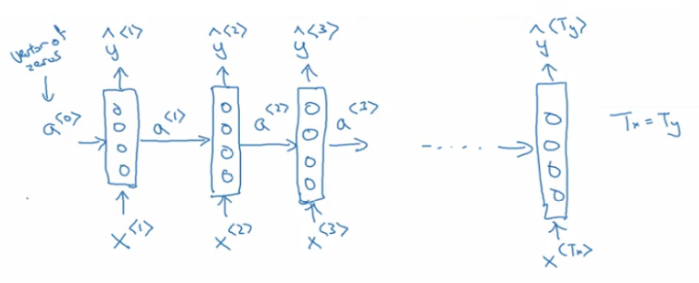
\includegraphics[width=1.0\textwidth]{img/c5/name-enttity-task.png}
    \caption{Example of name entity recognition task.}
    \label{name-entity}
\end{figure}

We should note:

\begin{itemize}
    \item In this problem, $T_x = T_y$. In other problems where thy aren't equal, the RNN architecture may be different.
    \item $a^{<0>}$ is usually initialized with zeros, but some others may initialize it randomly in some cases.
    \item There are three weight matrices here: $W_{ax}, W_{aa}$ and $W_{ya}$ with shapes: $W_{ax}\to (n_h, n_x), W_{aa}\to (n_h, n_h), W_{ya}\to (n_y, n_h)$.
\end{itemize}

The weight matrix $W_{aa}$ is the memory the RNN is trying to maintain from the previous layers.

In the discussed RNN architecture, the current output $y^{<t>}$ depends on the previous inputs and activations. 

Let's have this example `He Said, ``Teddy Roosevelt was a great president"'. In this example Teddy is a person name but we know that from the word \textit{president} that came after Teddy not from \textit{He} and \textit{said} that were before it.

So limitation of the discussed architecture is that it can not learn from elements later in the sequence. To address this problem we will later discuss \textbf{Bidirectional RNN (BRNN)}.

Now let's discuss the forward propagation equations on the discussed architecture (Figure \ref{forward-nn}):

\begin{figure}[!htbp]
    \centering
    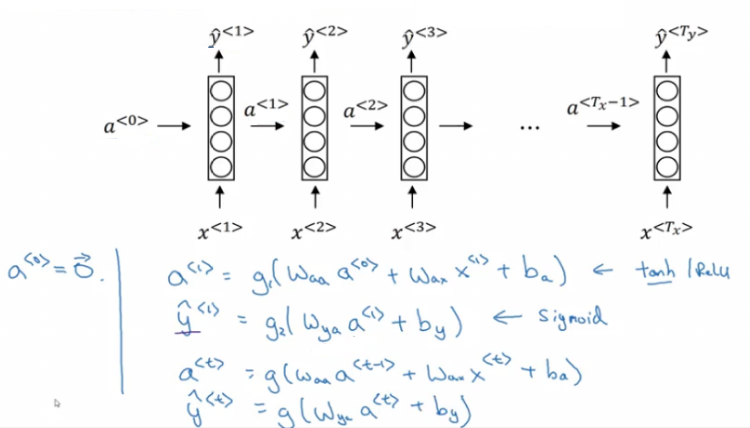
\includegraphics[width=1.0\textwidth]{img/c5/forward-rnn.png}
    \caption{Forward propagation of a RNN.}
    \label{forward-nn}
\end{figure}

The activation function for $a$ is usually $\tanh$ or $ReLU$ and for y depends on your task choosing some activation functions like $sigmoid$ and $softmax$. In name entity recognition task we will use sigmoid because we only have two classes.

In order to help us develop complex RNN architectures, the last equations needs to be simplified a bit (Figure \ref{simple-rnn-notations}):

\begin{figure}[!htbp]
    \centering
    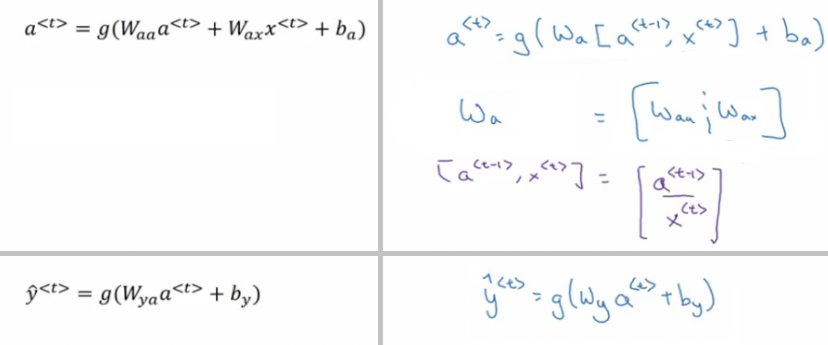
\includegraphics[width=1.0\textwidth]{img/c5/simple-rnn-notations.png}
    \caption{Simplified RNN notations.}
    \label{simple-rnn-notations}
\end{figure}

$w_a$ is $w_{aa}$ and $w_{ax}$ stacked horizontally. $[a^{<t-1>}, x^{<t>}]$ is $a^{<t-1>}$ and $x^{<t>}$ stacked vertically. $w_a$ shape: $(n_h, n_h+n_x)$. $[a^{<t-1>}, x^{<t>}]$ shape: $(n_h + n_x, 1)$.

\subsubsection{Backpropagation Through Time}
Usually deep learning frameworks do backpropagation automatically for you. But it's useful to know it works in RNNs.

We will use the cross-entropy loss function:

\begin{equation}
    L^{<t>}(\hat{y}^{<t>}, y^{<t>}) = - y^{<t>}\log \hat{y}^{<t>} - (1 - y^{<t>}) \log (1 - \hat{y}^{<t>})
\end{equation}

The total loss is:

\begin{equation}
    L(\hat{y}, y) = \sum_{t=1}^{T_y} L^{<t>}(\hat{y}^{<t>}, y^{<t>})
\end{equation}

The backpropagation here is called backpropagation through time because we pass activation a from one sequence element to another like backwards in time.

% Add more content of this part.

\subsubsection{Different Types of RNNs}
Here are different types of RNNs (Figure \ref{diff-rnns}, inspired by Andrej Karpathy's blog\footnote{http://karpathy.github.io/2015/05/21/rnn-effectiveness/}):

\begin{figure}[!htbp]
    \centering
    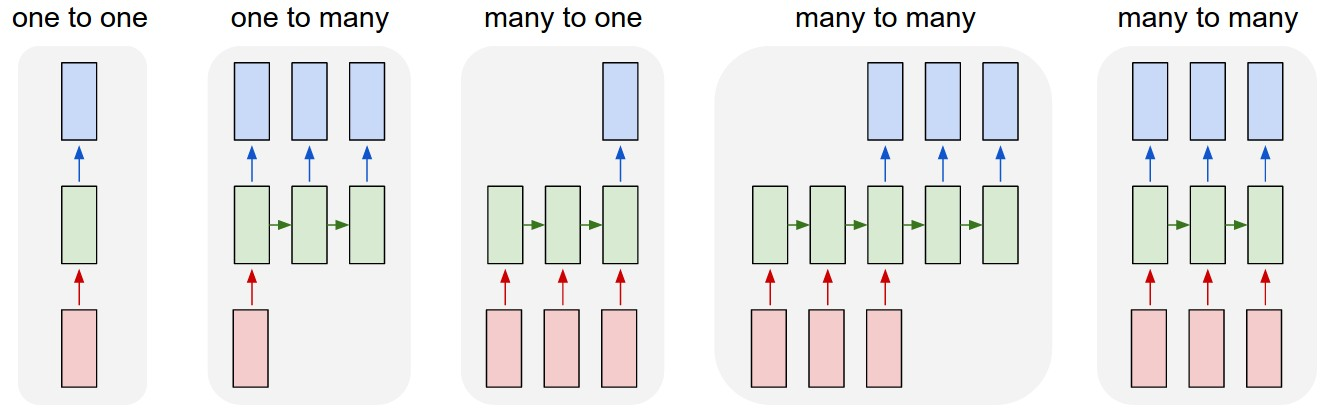
\includegraphics[width=1.0\textwidth]{img/c5/diff-rnns.jpg}
    \caption{Different kinds of RNNs.}
    \label{diff-rnns}
\end{figure}

\subsubsection{Language Model and Sequence Generation}
\textbf{What is a language model}:
\begin{itemize}
    \item Let's say we're solving a speech recognition problem and some says a sentence that can be interpreted into two sentences: a) The apple and \textit{pair} salad; b) The apple and \textit{pear} salad.
    \item \textit{Pair} and \textit{pear} sounds exactly the same, so how would a speech recognition application choose from the two.
    \item That's where the language model comes in. It gives a probability for the two sentences and the application decides the best based on this probability.
\end{itemize}

The job of a language model is to give a probability of any given sequence of words.

\textbf{How to build language models with RNNs}
\begin{itemize}
    \item The first thing is to get a training set: a large corpus of target language text.
    \item Then tokenize this training set by getting the vocabulary and then one-hot each word.
    \item Put an end of sentence token \textit{<EOS>} with the vocabulary and include it with each converted sentence. Also, use the token \textit{<UNK>} for the unknown words.
\end{itemize}

Given the sentence ``Cats average 15 hours of sleep a day. <EOS>"

In training time we will use this (Figure \ref{language-model}):

\begin{figure}[!htbp]
    \centering
    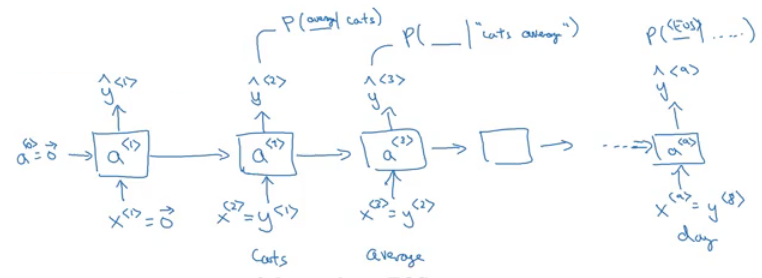
\includegraphics[width=1.0\textwidth]{img/c5/language-model.png}
    \caption{Example of language model.}
    \label{language-model}
\end{figure}

The loss function is defined by cross-entropy loss.

To use this model:
\begin{itemize}
    \item[i.] For predicting the chance of next word, we feed the sentence to the RNN and then get the final $y^{<t>}$ hot vector and sort it by maximum probability.
    \item[ii.] For taking the probability of a sentence, we compute this: $p(y^{<1>}, y^{<2>}, y^{<3>}) = p(y^{<1>}) * p(y^{<2>} | y^{<1>}) * p(y^{<3>} | y^{<1>}, y^{<2>})$. This is simply feeding the sentence into the RNN and multiplying the probabilities (outputs).
\end{itemize}

\subsubsection{Sampling Novel Sequences}
After a sequence model is trained on a language model, to check what the model has learned you can apply it to sample novel sequence.

To be continued.

% https://github.com/mbadry1/DeepLearning.ai-Summary/tree/master/5-%20Sequence%20Models#sampling-novel-sequences
\newpage